\documentclass[10pt]{article}
\usepackage[margin=0.75in]{geometry}
\usepackage[T1]{fontenc}
\usepackage{lmodern,microtype,booktabs,graphicx,xcolor,pgfplots,caption,float,amsmath}
\pgfplotsset{compat=1.18}
\usepgfplotslibrary{groupplots}
\captionsetup{font=small,skip=3pt}
\usepackage{titlesec}
\titleformat*{\section}{\large\bfseries}
\titlespacing*{\section}{0pt}{0.7em}{0.2em}
\setlength{\parskip}{0.4em}
\setlength{\parindent}{0pt}

% chart palette (validated: CVD-safe; aqua is below 3:1 on white, so every bar carries a value label)
\definecolor{maj}{HTML}{EB6834}
\definecolor{qwen}{HTML}{2A78D6}
\definecolor{nano}{HTML}{1BAF7A}
\definecolor{ink2}{HTML}{52514E}
\definecolor{grid}{HTML}{E4E3DF}
\pgfplotsset{
  every axis/.append style={axis line style={ink2!60}, tick style={draw=none},
    tick label style={font=\scriptsize, color=ink2}, label style={font=\scriptsize, color=ink2},
    ymajorgrids, grid style={grid, line width=0.4pt},
    legend style={draw=none, font=\scriptsize, text=ink2}, legend cell align=left, area legend},
  bars/.style={ybar=2pt, bar width=8pt, line width=0pt, draw=white,
    nodes near coords={\pgfmathprintnumber[fixed,precision=0]{\pgfplotspointmeta}},
    every node near coord/.append style={font=\tiny, color=black}},
}
\tikzset{chance/.style={dashed, ink2, line width=0.6pt}}

% GPT-4.1-nano accuracies (%), from src/score.py on Milestone 2/gpt-4.1-nano/*.jsonl
\newcommand{\NMD}{31.45}
\newcommand{\NMT}{33.90}
\newcommand{\NRD}{52.73}
\newcommand{\NRDE}{55.23}
\newcommand{\NRDH}{50.23}
\newcommand{\NRT}{54.79}
\newcommand{\NRTE}{55.74}
\newcommand{\NRTH}{53.83}

\title{\vspace{-3.5em}Cartoon Caption Matching and Humor Ranking\\\large CIS 4300/5300 Milestone 2: Evaluation and Baselines}
\author{Alex Yang, Maggie Du, Celia Tung, Chinmay Govind}
\date{November 18, 2026}

\begin{document}
\maketitle
\vspace{-2.5em}

\section{Tasks and data}
We test whether models get New Yorker cartoon humor with 2 multiple-choice tasks. In \textbf{matching}, the model sees a cartoon and 5 captions and picks the one that was actually written for it (chance is 20\%). In \textbf{ranking}, it sees a cartoon and 2 contest entries and picks the one the crowd rated funnier (chance is 50\%). Matching comes from Hessel et al.~[1]; ranking pairs come from the crowd ratings released by Zhang et al.~[2]. Easy pairs put a top-10 caption against one ranked 1000-1009, and hard pairs put rank 30-39 against rank 300-309. \par

\begin{figure}[H]
\centering
\begin{minipage}[c]{0.22\linewidth}\centering
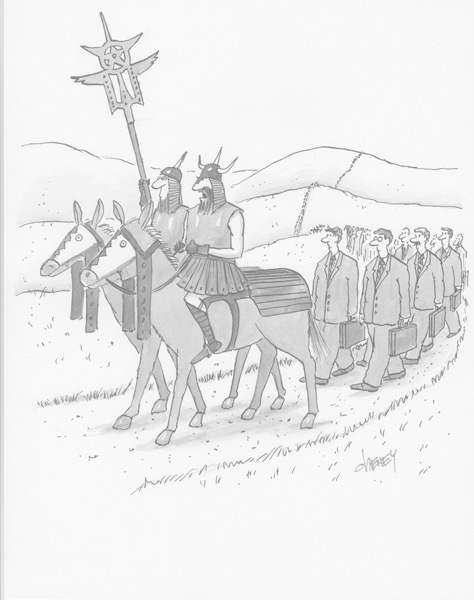
\includegraphics[width=\linewidth]{cartoon575.jpg}
\end{minipage}\hfill
\begin{minipage}[c]{0.75\linewidth}\small
\textbf{Matching} (test item, contest 575). Which caption belongs to this cartoon?\\
A: ``Evolution can be so tacky.'' \quad
\textbf{B: ``Let's pick up the pace. They're billing by the hour.''} (correct)\\
C: ``Well, five acres of popcorn back there says you were.'' \quad
D: ``I'm sure it works. I was involved in the original research.'' \quad
E: ``Just water for me, thanks.''\par
\medskip
\textbf{Ranking} (hard pair, contest 575). Which caption did the crowd like more?\\
\textbf{A: ``You're the one who wanted to negotiate.''} (rank 30, correct)\\
B: ``Remember, the lawyers go into battle first. That way we'll be popular whether we win or lose.'' (rank 300)
\end{minipage}
\caption{One cartoon, both tasks. Qwen got the matching item right and the ranking pair wrong (it picked B).}
\end{figure}
\vspace{-1em}

\begin{center}\small
\begin{tabular}{lrrr}
\toprule
Items (contests) & Train & Dev & Test \\
\midrule
Matching & 4,896 (422) & 531 (141) & 528 (141) \\
Ranking & 5,420 (271) & 880 (44) & 940 (47) \\
\bottomrule
\end{tabular}
\end{center}
\vspace{-0.5em}
No contest shows up in more than one split, so the model never gets tested on a cartoon it trained on. \par

\section{Evaluation measure}
Both tasks have exactly one right answer per item, so we use accuracy, the same metric Hessel et al.~[1] report for matching. For ranking, accuracy on a pair is just whether the model agreed with the crowd. For $N$ items with ground truth labels $y_i$ and system predictions $\hat{y}_i$,
$$\text{Acc} = \frac{1}{N}\sum_{i=1}^{N} \mathbf{1}[\hat{y}_i = y_i].$$
A prediction that is missing or can't be parsed into a letter counts as wrong. For ranking we also report accuracy on the easy and hard pairs separately. Our scorer takes a ground truth file and a predictions file and lines them up by item ID: \par
\vspace{-0.3em}
{\small\verb|python src/score.py "Milestone 1/data/ranking/test.jsonl" predictions.jsonl|}\par

\section{Simple baseline: majority class}
The simplest system ignores the cartoon and the captions completely. It just finds the most common answer letter in the training set and predicts it for every item:
$$\hat{y}(x) = \arg\max_{c} \sum_{i \in \text{train}} \mathbf{1}[y_i = c].$$
So, it always says E for matching (1,031 of 4,896 training labels) and B for ranking (2,760 of 5,420). It scores \textbf{18.37\%} on matching test and \textbf{50.00\%} on ranking test, which is basically chance. \par

\section{Strong baselines: zero-shot vision-language models}
Our strong baseline adapts the zero-shot setup in Hessel et al.~[1]: show a vision-language model the raw cartoon and the lettered captions, then ask for exactly one letter. There's no fine-tuning and no examples in the prompt. Both models below get the exact same prompt, and we decode greedily. Any reply that isn't a single valid letter is marked wrong. \par

\textbf{Qwen3.5-4B} [3] is a small open-weight model, which we ran on an NVIDIA L4 in Colab. Images were capped at 512$\times$512 pixels and thinking was turned off. \par

\textbf{GPT-4.1-nano} [4] is OpenAI's cheapest vision model, which we called through Azure OpenAI with temperature 0. Images were sent at the API's \texttt{low} detail setting, which is also 512$\times$512, so both models see the cartoon at about the same resolution. Each item is only about 600 input tokens, so all 2,879 dev and test items cost roughly \$0.20. \par

\section{Results}
\begin{figure}[H]
\begin{minipage}[c]{0.43\linewidth}\centering\small
\begin{tabular}{@{}llrrr@{}}
\toprule
Task & Split & Maj. & Qwen & nano \\
\midrule
Matching & dev  & 19.77 & 47.27 & \NMD \\
Matching & test & 18.37 & 49.62 & \NMT \\
\midrule
Ranking & dev  & 48.98 & 50.80 & \NRD \\
\quad easy & dev & 45.91 & 48.41 & \NRDE \\
\quad hard & dev & 52.05 & 53.18 & \NRDH \\
Ranking & test & 50.00 & 51.49 & \NRT \\
\quad easy & test & 50.85 & 52.77 & \NRTE \\
\quad hard & test & 49.15 & 50.21 & \NRTH \\
\bottomrule
\end{tabular}
\end{minipage}\hfill
\begin{minipage}[c]{0.55\linewidth}\centering
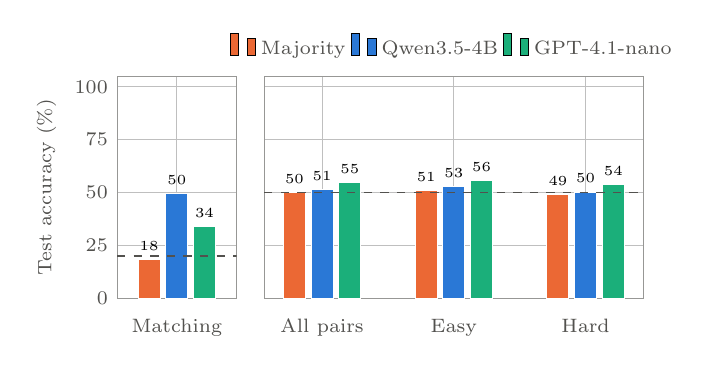
\begin{tikzpicture}
\begin{groupplot}[group style={group size=2 by 1, horizontal sep=0.35cm, yticklabels at=edge left},
  height=4.4cm, ymin=0, ymax=105, ytick={0,25,50,75,100}, bars]
\nextgroupplot[width=3.1cm, symbolic x coords={Matching}, xtick=data, enlarge x limits=1.2, ylabel={Test accuracy (\%)}]
  \addplot[fill=maj] coordinates {(Matching,18.37)};
  \addplot[fill=qwen] coordinates {(Matching,49.62)};
  \addplot[fill=nano] coordinates {(Matching,\NMT)};
  \draw[chance] ({rel axis cs:0,0}|-{axis cs:Matching,20}) -- ({rel axis cs:1,0}|-{axis cs:Matching,20});
\nextgroupplot[width=6.4cm, symbolic x coords={All pairs,Easy,Hard}, xtick=data, enlarge x limits=0.22,
  legend style={at={(0.5,1.03)}, anchor=south}, legend columns=3]
  \addplot[fill=maj] coordinates {(All pairs,50.00) (Easy,50.85) (Hard,49.15)};
  \addplot[fill=qwen] coordinates {(All pairs,51.49) (Easy,52.77) (Hard,50.21)};
  \addplot[fill=nano] coordinates {(All pairs,\NRT) (Easy,\NRTE) (Hard,\NRTH)};
  \draw[chance] ({rel axis cs:0,0}|-{axis cs:Easy,50}) -- ({rel axis cs:1,0}|-{axis cs:Easy,50});
  \legend{Majority, Qwen3.5-4B, GPT-4.1-nano}
\end{groupplot}
\end{tikzpicture}
\end{minipage}
\caption{Accuracy (\%) of every baseline, all computed by \texttt{src/score.py} from saved prediction files. Left: every split. Right: test accuracy for matching and ranking; the dashed line is chance.}
\end{figure}
\vspace{-0.8em}

So, neither strong baseline wins both tasks. Qwen is far better at matching: 49.62\% on test against nano's 33.90\%, though both clear the 20\% chance line. Ranking flips it. Nano gets 54.79\% on test and is the only system meaningfully above the majority baseline, while Qwen sits at 51.49\%. Nano also does worse on hard pairs than easy ones (53.83\% vs.\ 55.74\% on test, 50.23\% vs.\ 55.23\% on dev), which makes sense: ranks 30 and 300 are much closer in quality than ranks 1 and 1000. \par

Both models lean on answer position instead of the captions. Qwen answered B on 826 of 940 ranking test pairs (87.87\%), even though the ground truth labels are split exactly 470/470. Nano's bias is milder and points the other way: it answered A on 591 pairs (62.87\%). Azure's content filter also blocked cartoons 222 and 617 outright, so nano lost 5 matching items and 17 ranking pairs before it ever saw them; those count as wrong. \par

\textbf{Next steps.} Since position bias is the biggest problem on ranking, our first extension will score every pair in both orders and only count a caption as preferred if the model picks it both times. \par

\vspace{-0.5em}
{\small
\textbf{References}\\
{[1]} Hessel et al. 2023. Do Androids Laugh at Electric Sheep? Humor ``Understanding'' Benchmarks from The New Yorker Caption Contest. ACL.\\
{[2]} Zhang et al. 2024. Humor in AI: Massive Scale Crowd-Sourced Preferences and Benchmarks for Cartoon Captioning. NeurIPS Datasets and Benchmarks.\\
{[3]} Qwen Team. 2026. Qwen3.5. \texttt{huggingface.co/Qwen/Qwen3.5-4B}.\\
{[4]} OpenAI. 2025. GPT-4.1 model family. \texttt{openai.com/index/gpt-4-1}.\par}

\end{document}
